\documentclass[12pt,a4paper,oneside, openany]{book}


\usepackage{lmodern}
\usepackage[table]{xcolor}
\usepackage{xcolor}
\definecolor{vert1}{rgb}{0.0,0.3.9,0.0}
\definecolor{bleu}{rgb}{0,0,0.5}
\definecolor{bleu3}{rgb}{1,0.2,0.2}
\definecolor{grisgris}{gray}{0.4}
\definecolor{grisclair}{HTML}{E7E7E7}
\definecolor{grisfonce}{HTML}{A5A5A5}
\definecolor{rougeUPS}{rgb}{0.6, 0.3, 0.3}

\fboxsep =0pt \parindent =0pt\parskip =12pt



\usepackage[utf8]{inputenc}
\usepackage[T1]{fontenc}
\usepackage[francais]{babel}
\usepackage[top=1.7cm, bottom=1.7cm, left=1.7cm, right=1.7cm]{geometry}
\usepackage{verbatim}
\usepackage[urlbordercolor={1 1 1}, linkbordercolor={1 1 1}, linkcolor=vert1, urlcolor=bleu, colorlinks=true]{hyperref}
\usepackage{tikz} %Vectoriel
\usepackage{listings}
\usepackage{fancyhdr}
\usepackage{multido}
\usepackage{amssymb}
\usepackage{eurosym}
\usepackage{array}
\usepackage{float}
\usepackage{graphicx}

\newcommand{\US}{User Story}
\newcommand{\USs}{User Stories}

\newcommand{\story}[1]{ User story ``\textit{#1}'' }

\newcommand{\footnotesouvenir}[2]{
	\footnote{#2}
	\newcounter{#1}
	\setcounter{#1}{\value{footnote}}
}
\newcommand{\footnoterappel}[1]{
	\footnotemark[\value{#1}]
}

\newcommand{\remarque}[1]{
	\begin{center}
	\medskip
	\colorbox{remarque}{
		\begin{minipage}{0.85\textwidth}\medskip
\includegraphics[height=10px]{images/remarque.png} #1 \medskip\end{minipage}
	}
	\medskip
	\end{center}
}

\newcounter{exemples}

\newenvironment{exemple}[1]{
   \vspace{-2mm}

\refstepcounter{exemples}
   \begin{center}
	\medskip
      \begin{minipage}{0.9\linewidth}
}{%
~
      \end{minipage}
   \end{center}~
   \vspace{-2mm}
}%

\newcommand{\captionExemple}[1]{
	\begin{center}{\bsc{Exemple} \thechapter.\arabic{exemples}~--~}#1\end{center}
}


\DeclareTextFontCommand{\policeGlossaire}{\fontfamily{lmss}\selectfont}
\DeclareTextFontCommand{\policePackage}{\fontfamily{phv}\selectfont}
\DeclareTextFontCommand{\policeTitre}{\fontfamily{ptm}\selectfont}
\newcommand{\policeCode}[1]{\texttt{#1}}

\newcommand{\sectionfont}{%
	\fontencoding{\encodingdefault}%
	\fontfamily{pag}%
	\fontseries{bc}%
	\fontshape{n}%
	\selectfont
}

% numéro du chapitre
\DeclareFixedFont{\chapnumfont}{T1}{phv}{b}{n}{80pt}
% pour le mot « Chapitre »
\DeclareFixedFont{\chapchapfont}{T1}{phv}{b}{n}{16pt}
% pour le titre
\DeclareFixedFont{\chaptitfont}{T1}{phv}{b}{n}{24.88pt}


\usepackage{ifthen}

\newsavebox{\fmbox}
\newenvironment{fmpage}[1]
     {\begin{lrbox}{\fmbox}\begin{minipage}{#1}}
	  {\end{minipage}\end{lrbox}\fbox{\usebox{\fmbox}}}


\makeatletter

\title{Projet Agile --- \bsc{SCRUM}}

\def\top#1{\def\@top{#1}}

\def\sousTitre#1{\def\@sousTitre{#1}}
\sousTitre{Rubidium}

\def\location#1{\def\@location{#1}}
\location{Toulouse}

\date{\today}

%% Entete (Université..)  
\def\clap#1{
	\hbox to 0pt{\hss #1\hss}
}%
\def\ligne#1{%
	\hbox to \hsize{%
		\vbox{\centering #1}
	}
}%

% définition du haut de la couverture %
\def\haut#1#2#3{%
	\hbox to \hsize{%
		\rlap{
			\vtop{\raggedright #1}
		}%
		\hss
		\clap{	
			\vtop{\centering #2}
		}%
		\hss
		\llap{
			\vtop{\raggedleft #3}
		}
	}
}%

% Définition du bas de la couverture %
\def\bas#1#2#3{%
	\hbox to \hsize{%
	\hss \clap{\vbox{
	\centering \hspace{1.7cm}\newline
		\newline \newline \newline	\newline \newline \newline	\newline \newline \newline	\newline \newline \newline	\newline \newline \newline	\newline \newline \newline\newline #2 }
		}%
		\hss
	}
}%

% Zou, on peut construire la page de garde 
\def\maketitle{%
	\thispagestyle{empty}\vbox to \vsize{%
		\vspace{-25px}
		\vspace{5px}
		\haut{}{\@top}{}
		\vfill
		\begin{flushleft}
			David \bsc{Bernard}\\
			Mathias \bsc{Faure}\\
			Antoine \bsc{Incorvaia}\\
			Lucas \bsc{Le gouic}\\
			Antoine de \bsc{Roquemaurel}\\
			Clément \bsc{Vannier}\\
		\end{flushleft}

		\begin{flushright}
			\vspace{-3cm}
			\begin{tabular}{r@{~}l}
				Pour M. \bsc{Fernandez} 
			\end{tabular}
		\end{flushright}
		\vfill
		\vspace{1cm}
		\begin{flushleft}
			\policeTitre{\huge \@title}
		\end{flushleft}

		\par
		\hrule height 4pt
		\par

		\begin{flushright}
			\policeTitre{\Large \@sousTitre}
			\par
		\end{flushright}
		\vspace{3.2cm}
		\bas{}{ \@location, le \@date}{}
		\vspace{5px}
		\vspace{-15px}
	}%
	\cleardoublepage
}

\makeatother

\top{%
	Université Paul Sabatier -- Toulouse III\\
	IUT A - Toulouse Rangueil\\
	%\textbf{Projet tuteuré \#20}\\[1em]
}%

\makeatletter

\makeatother
\pagestyle{fancy}

\makeatletter
\def\thickhrulefill{\leavevmode \leaders \hrule height 1ex \hfill \kern \z@}
%% \chapter
\def\@makechapterhead#1{%
  \reset@font
  \parindent \z@
  \vspace*{10\p@}%
  \hbox{%
    \vbox{%
      \advance\hsize by -2cm
      \hrule height 0.4pt depth 0pt width \hsize
      \par
      \vskip 6pt%
      \hspace{20pt}%
      \parbox{420pt}{%
        \LARGE \bfseries #1
		}%
      \par
      \vskip 6pt%
      \hspace{20pt}%
      \hrule height 0.4pt depth 0pt width \hsize
	  \vspace{-30pt}
      }%
    \vbox{%
      \hsize=1.5cm%
      \begin{tabular}{c}
        \scshape \large \strut \@chapapp{} \\
        \colorbox{black}{\vbox{\hbox{\vbox to 1mm{}}\hbox{
			\color{white} \LARGE \bfseries \hspace{1mm}\thechapter\hspace{1mm}
		}\hbox{\vbox to 2cm{}}}}%
      \end{tabular}%
      }%
    }%
  \vskip 20\p@
}
%% \chapter*
\def\@makeschapterhead#1{%
  \reset@font
  \parindent \z@
  \vspace*{10\p@}%
  \hbox{%
    \vbox{%
      \advance\hsize by -0cm
      \hrule height 0.4pt depth 0pt width \hsize
      \par
      \vskip 6pt%
      \hspace{20pt}%
      \parbox{420pt}{%
        \LARGE \bfseries #1
		}%
      \par
      \vskip 6pt%
      \hspace{20pt}%
      \hrule height 0.4pt depth 0pt width \hsize
      }%
    }%
  \vskip 20\p@

}

\newlength{\sectiontitleindent}
\newlength{\subsectiontitleindent}
\newlength{\subsubsectiontitleindent}
\setlength{\sectiontitleindent}{-1cm}
\setlength{\subsectiontitleindent}{-.5cm}
\setlength{\subsubsectiontitleindent}{-.25cm}

\renewcommand{\section}{%
	\@startsection%
	{section}%
	{1}%
	{\sectiontitleindent}%
	{-3.5ex plus -1ex minus -.2ex}%
	{2.3ex plus.2ex}%
	{\sectionfont\Large}
}
\renewcommand{\subsection}{%
	\@startsection%
	{subsection}%
	{2}%
	{\subsectiontitleindent}%
	{-3.5ex plus -1ex minus -.2ex}%
	{2.3ex plus.2ex}%
	{\sectionfont\large}
}

\renewcommand{\subsubsection}{%
	\@startsection%
	{subsubsection}%
	{3}%
	{\subsubsectiontitleindent}%
	{-3.5ex plus -1ex minus -.2ex}%
	{2.3ex plus.2ex}%
	{\sectionfont\normalsize}
}

\makeatother



\lhead{Projet Agile --- \bsc{Scrum}}
\cfoot{\thepage}





\includeonly{
includes/documentDeSynthese,
includes/chapitre1, 
includes/chapitre2,
includes/chapitre3,
includes/chapitre4,
includes/chapitre5,
includes/chapitre6,
includes/annexes/glossaire,
includes/annexes/listeAnnonceurs,
includes/annexes/listeTableauxCh6
}

\begin{document}
	\setcounter{tocdepth}{1}
	\setcounter{secnumdepth}{3}
	\maketitle
	\frontmatter
	\chapter*{Document de synthèse}
	\addcontentsline{toc}{chapter}{Document de synthèse}
	\paragraph{}
	La société \K{} (Logo figure \ref{fig:logo}) conçoit des solutions logicielles pour les 
	\glo{TPE}{TPE}{Les très petites entreprises (TPE) sont en France une appellation des entreprises de moins de 20 salariés}\footnote{\textbf{T}rès \textbf{P}etites \textbf{Entreprises}} et 
	les \glo{PME}{PME}{Les petites et les moyennes entreprises sont des entreprises dont la taille, définie à partir du nombre d'employés, du bilan ou du chiffre d'affaires, ne dépasse pas certaines limites ; les définitions de ces limites diffèrent selon les pays.}\footnote{\textbf{P}etites et \textbf{M}oyennes \textbf{E}ntreprises} du \glo{génie climatique}{Génie climatique}{
Le génie climatique est une branche de la physique qui traite du domaine du chauffage, de la plomberie, de la climatisation et du gaz et de ses applications. L'étude de domaine se réalise en physique, l'application se fait dans le domaine industriel.}. 
	Une des problématiques de ce secteur est la réalisation d’un bilan thermique précis.\\
	À l'heure actuelle, les professionnels n'ont à leu disposition que peu d'outils :
	\begin{itemize}
		\item Tableurs Excel réalisés en interne
		\item Logiciels réglementaires très couteux (plusieurs milliers d'euros)
	\end{itemize}

	Dans le premiers cas, les résultats sont approximatifs et dans le contexte actuel de maitrise 
	de l'énergie, il devient primordial de pouvoir réaliser ces calculs de façon précise.\newline
	Au niveau des logiciels payants, les calculs sont précis mais leur prix reste un obstacle à 
	leur utilisation pour la quasi totalité des entreprises visées.  De plus, l'ergonomie de ces 
	outils les rend difficile d’usage.

	\paragraph{}
	L'idée de ce projet est née à travers diverses expériences dans le secteur du génie climatique.
	Une première tentative avait été menée durant l'été 2009. Ce projet avait été soutenu par des 
	professionnels (entreprise A.S.O à Toulouse) qui avait mis à disposition des locaux et avait 
	fait une proposition d’actionnariat. Cependant, le projet n’a pas pu être mené à son terme par 
	manque de temps et d’organisation.\\
	Le projet a été relancé en octobre 2010, à la suite de divers échanges avec des professionnels.

	\paragraph{}
	Aujourd'hui une nouvelle équipe a été formée et une nouvelle méthode de calcul a été adoptée.

	\paragraph{}
	L'objectif est de distribuer gratuitement les solutions logicielles proposées par \K{} qui 
	seront téléchargeables sur le site internet de la société.  En contre partie, des encarts 
	publicitaires seront réservés aux fabricants de système de chauffage et de climatisation sur 
	la fenêtre d’accueil (splach screen) et sur la fenêtre principale du logiciel.

  \begin{figure}[H]
	  \begin{center}
	\includegraphics[width=3.6cm]{images/logo.png}
	  \end{center}
	  \caption{Logo de \K{}}
	  \label{fig:logo}
  \end{figure}


	\tableofcontents
	\mainmatter
	\chapter{Introduction}
	\section{Complexité}
	On cherche à estimer le temps de calcul d'un algorithme A en fonction d'un paramètre n. Pour avoir une mesure indépendante de la machine, on identifie
	le temps de calcul avec le nombre d'instructions exécutées. 
	
	\exemple{Le paramètre n pourrait être la taille d'un tableau, par exemple.}

	Soit $D_i$ l'ensemble des données possibles telle que $n=i$. Pour $d \in D_i$ on notera $T(A,d)$ le nombre d'instructions exécutée pendant l'exécution de
	$A(d)$.\\
	On notera $\prob(d|i)$ la probabilité que les données soit $d$ étant donné qu'elles sont de taille $i$.

	\subsection{La complexité temporelle maximale} 
	La complexité temporelle maximale\footnote{Complexité dans le pire des cas} d'un algorithme A :
	$$T_{\max}(i) = \max_{d\in D_i}\{T(A,d)\}$$
	\subsection{La complexité temporelle moyenne}
	La complexité temporelle moyenne\footnote{Complexité dans le cas moyen} d'un algorithme A :
	$$T_{\moy} = \sum_{d \in D_i} \prob(d|i) \times T(A,d)$$
	\remarque{Pour pouvoir calculer $T_\moy$, il faut connaître la distribution des données, ce qui n'est pas toujours évident (par exemple en traitement d'image)}
	\subsection{La complexité temporelle minimale}
	La complexité temporelle minimale\footnote{Complexité dans le meilleur des cas} d'un algorithme A :
	$$T_{\min}(i) = \min_{d\in D_i}\{T(A,d)\}$$ 
	\remarque{Peu utilisé, sauf pour prouver qu'un algorithme est mauvais. Si la complexité temporelle minimale est 
		mauvaise même dans le meilleur des cas, alors l'algorithme n'est pas bon.}

%			\remarque{$T_{\max}$ et $T_{\min}$ nous fournissent des bornes supérieures et inférieures.}

	\subsection{Compairaison de complexités en fonction de la machine}
	\begin{tabular}{| c | p{7cm} | p{7cm}|} 
		\hline
		\textbf{Complexité}& \multicolumn{2}{|c|}{\textbf{Nombre d'instructions pouvant executer la machine}}\\
		\hline
		 & $1\;000\;000$ & $1\;000\;000\;000\;000$\\
		\hline
		$n$ & $1\;000\;000$&$1\;000\;000\;000\;000$\\
		\hline
		$n \log_2 n$ &$64\;000$&$32\;000\;000\;000$\\
		\hline
		$n^2$ & $1\;000$&$1\;000\;000$\\
		\hline
		$n^3$ &$100$&$10\;000$\\
		\hline
		$2^n$ &$20$&$40$\\
		\hline
	\end{tabular}
	\section{Complexité asymptotique}
	Pour comparer des algorithmes, on ne s'intéresse qu'à leur comportements pour n grand. On cherche une mesure de complexité qui soit indépendante du langage de programmation et de la vitesse de la machine. \\ 
$\Rightarrow$		On ne doit pas perdre en compte des facteurs constants.  \\
$\Rightarrow$	Ordre de grandeur

\subsection{La complexité asymptotique}
La complexité asymptotique\footnote{Que ce soit maximale, moyenne ou minimale} est l'ordre de grandeur de sa limite lorsque $n \rightarrow \infty$

\subsection{Notation} Soient $T$, $f$ des fonctions positives ou nulles. Rotations de grandeur de fonction asymptotiques.
\paragraph{Grand O} $T = O(f)$ si $\exists c \in \mathbb{R}^{>0}$ et $n_0 \in \mathbb{N}$ tels que $\forall n \geq n_0$, $T(n) \leq cf(n)$.

\paragraph{Grand Oméga} $T = \Omega(f)$ si $\exists c \in \mathbb{R}^{>0}$ et $n_0 \in \mathbb{N}$ tels que $i\forall n \geq n_0$, $T(n) \geq cf(n)$
\paragraph{Petit O} $T = o(f)$ si $\frac{T(n)}{f(n)} \rightarrow O$ lorsque $n \rightarrow \infty$. 
\remarque{T est négligeable devant f}

\exemple{
\begin{enumerate}
	\item $2n^2 + 5n + 10 = O(n^2)$\\
	Dans la définition $n_0 = 5$,$c=4$ : \\
	$\forall n \geq 5,\ 2n^2+5n+10 \leq 4n^2$
\item $2n^2 + 5n + 10 = \Omega(n^2)$\\
	Dans la définition, $n_0 = 1$, $c = 2$\\
	$\forall n \geq 1,\ 2n^2 + 5n + 10 \geq 2n^2 \cdots$\\
	Donc $2n^2+5n+10 = \Theta (n^2)$
\item $\frac{1}{5} + n = O(n\log_2 n)\ (n_0 = 2,\ c=2)$
\item $\frac{1}{5} n \log_2 n + n = \Omega(n \log n)\ (n_0=1,c=\frac{1}{5})$
\item $\forall k \geq 0$, $n^k = O(n^{k+1})$ mais $n^k \neq \Omega(n^{k+1})$
\item $\forall a,b >1, \log_a n = \Theta (\log_b n)$ car $\log_a n = \frac{\log_b n}{\log_b a}$ et $\log_b a$ est une constante. $\Rightarrow$ On a pas besoin de préciser la base de logarithme dnas une complexité asymptotique
\item $2n^2 + 5n + 10 = 2n^2 + 0(n^2)$
\item Pour toute constante $c>0$, $C = \Theta(1)$
\item $2^n = o(3^n)$
\end{enumerate}
}
\remarque{\begin{enumerate}
	\item O et $\Omega$ sont des pré-ordres\footnote{Relations reflexives et transitives} :\\ $f = O(f)$ et $f = O(g)$ et $g = O(h)) \Rightarrow f = O(h)$
	\item $\Theta$ est une relation d'équivalence\footnote{relation reflexives, symétrique et transitive} : 
		$f = \Theta(g) \Leftrightarrow g = \Theta (f)$
\end{enumerate}
}
\paragraph{Proposition}
$$\textrm{Si } \lim_{n \rightarrow \infty} \frac{f(n)}{g(n)} = a > 0 \textrm{ Alors }f = \Theta (g)$$
\remarque{La réciproque est fausse}

\paragraph{Notation} $$f \sim g \Rightarrow \lim_{n\rightarrow \infty} \frac{f(n)}{g(n)} = 1$$
\exemple{$(3n+1)^3 \sim 27n^3$}
\section{Exemple de complexités d'algorithmes}
\subsection{Le tri à bulles}
\begin{eqnarray*}
	T_{\min} (n) &=& \Theta (n) \textrm{ Si le tableau est est déjà trié}\\
	T_{\max}(n) &=& \Theta(n^2) \textrm{ Si le tableau est trié en ordre décroissant}\\
	T_{\moy}(n) &=& T_{\max}(n) = \Theta(n^2)\\
\end{eqnarray*}
\subsection{Tri par fusion}
\begin{eqnarray*}
	T_{\min}(n) = T_{\max}(n) = T_{\moy}(n) = \Theta (n\log n)
\end{eqnarray*}
\subsection{Tri rapide}
\begin{eqnarray*}
	T_{\min}(n) = T_{\moy}(n) &=& \Theta (n \log n)\\
	T_{\max}(n) &=& \Theta(n^2)
\end{eqnarray*}

\section{Comportement symptotique de fonctions usuelles}
Il y a quatre groupes importants de fonction positives croissantes.
\begin{description}
	\item[Logarithmiques] $(\log n)^\sigma$ (où $\sigma > 0$), $\log\log n, \ldots$
	\item[Polynomiales] $n^\gamma$ (où $\gamma > 0$), $n^\gamma(\log n)^\gamma$(où $\gamma > 0$)
	\item[Exponentielles] $2^{\alpha n^\beta}$ (où $\alpha > 0$ et $0 < \beta \leq 1$), par exemple $2^n$, $4^n$, $2^{\sqrt{n}}$
	\item[Supraexponentielles] $n!$, $n^n$, $2^{n^2}$, \ldots
\end{description}
\remarque{
	Il existe des fonctions intermédiaires(par exemple $n^{\log_2 n}$) mais ces fonctions se rencontrent très rarement dans l'analyse de complexité d'algorithmes
}

% Courbes. CF Feuille de TD
\begin{eqnarray*}
	\lim_{n\rightarrow \infty} \frac{n^b}{a^n} = O \textrm{ Pour toutes constantes} a,b \textrm{ avec } a > 1 \textrm{)}\\
	n^b = o(a^n)\\
	\lim_{n\rightarrow \infty} \frac{(\log_2 n)^{\sigma}}{n^\sigma} = O\\
	\Rightarrow (\log_2 n)^\sigma = o(n^\sigma)\\
\end{eqnarray*}


\subsection{La formule de Stisling}
\begin{eqnarray*}
	n! \sim \sqrt{2\pi n}(\frac{n}{e})^n\\
	\Rightarrow n! = o(n^n) \textrm{ et } n! = \Omega(2^n)
\end{eqnarray*}
On peut aussi en déduire :
$$\log(n!) \sim n\log n$$


		\chapter{Imbrication -- Ensembliste}
	\remarque{Interdiction d'utiliser les jointures}
	\begin{enumerate}
		\item 
				$R = \Pi_{nome} (\sigma_{ne\ \in\ (\Pi_{ne}\ Projet)})$\\
	\begin{lstlisting}[language=SQL, numbers=none]
select distinct nome from equipe e1 
where e1.ne in (select distinct ne from projet); 
	\end{lstlisting}

\item 
	$ R = \Pi_{nomc}(\sigma_{nc \in\ (\Pi_{nc}(\sigma_{np = 'p1'}aff)})Chercheur)$
	\begin{lstlisting}[language=SQL, numbers=none]
select distinct nomc from chercheur
where nc in (select distinct nc from aff where np='p1');
	\end{lstlisting}
\item 
	\begin{eqnarray*}
	R &=& \Pi_{nomc}(\sigma_{nc\ \in R_1} chercheur)\\
	R_1 &=& \Pi_{nc}(\sigma_{np\ \in\ R_2} aff)\\
	R_2 &=& \Pi_{np}(\sigma_{ne = 'e1'} Projet)
	\end{eqnarray*}
	\begin{lstlisting}[language=SQL, numbers=none]
select distinct nomc from chercheur 
where nc IN (select nc from aff 
						where np in (select np from projet where ne = 'e1'));
	\end{lstlisting}
\item 
	$\Pi_{nomc} (\sigma_{nc\ \in\ (\Pi_{nc}\ aff)} chercheur)$
	\begin{lstlisting}[language=SQL, numbers=none]
select distinct nomc from chercheur where nc in (select distinct n from aff);
	\end{lstlisting}
\item 
	$\Pi_{nomc} (\sigma_{nc\ \notin\ (\Pi_{nc}\ aff)} chercheur)$
	\begin{lstlisting}[language=SQL, numbers=none]
select distinct nomc from chercheur where nc not in (select distinct n from aff);
	\end{lstlisting}
\item ~ 
	\remarque{À partir de cette question la notation algébrique n'est pas indispensable.\\
	L'utilisation des opérateurs ensembliste est indispensable, chercher ensuite une requete non ensembliste}
	\begin{lstlisting}[language=SQL, numbers=none]
select nomc from chercheur where nc in (
	select ne from aff 
	where np in(select np from projet where nomp = 'SRI')
)
intersect
select nomc from chercheur where nc in (
	select ne from aff 
	where np in(select np from projet where nomp = 'BIG')
)
	\end{lstlisting}
\item ~ 
	\begin{lstlisting}[language=SQL, numbers=none]
(select nomc from chercheur where nc in (
	select ne from aff 
	where np in(select np from projet where nomp = 'SRI')
)
intersect
select nomc from chercheur where nc in (
	select ne from aff 
	where np in(select np from projet where nomp = 'BIG')
))
except
(select nomc from chercheur where nc in (
	select ne from aff 
	where np in(select np from projet where nomp <> 'SRI' and nomp <> 'BIG')
)
);
	\end{lstlisting}
\end{enumerate}

\chapter{Jointure}
\begin{enumerate}
	\item 
	\begin{lstlisting}[language=SQL, numbers=none]
select ne, nome, pbudget from equipe, projet 
where equipe.ne = projet.ne and equipe.ne = 'e1';
	\end{lstlisting}
\item ~ 
	\begin{lstlisting}[language=SQL, numbers=none]
select nomc, nome from equipe, chercheur, aff 
where aff.nc = chercheur.nc and aff.ne = equipe.ne;
	\end{lstlisting}
\item ~
	\begin{lstlisting}[language=SQL, numbers=none]
select count(nc) from equipe, aff group by equipe,aff having equipe.nc = aff.nc
	\end{lstlisting}
\end{enumerate}



	\chapter{Méthodologie de la programmation impérative}
\minitoc
	\section{Les différents types de problèmes}
		\subsection{Programmation <<en petit>>}
		\begin{description}
			\item[Données] celle-ci son simple, comme un tableau à N éléments.
			\item[Problème] Petit.
			\item[Résolution] Développement d'un algorithme afin de traiter ces données.
		\end{description}
		Cf. cours du S3.

		\subsection{Programmation en large}
		\begin{description}
			\item[Données] celle-ci son complexes, modélisation des données avec des types abstrait.
			\item[Résolution] Développer de nombreux algorithmes afin de traiter le type abstrait. 
		\end{description}
		Cf. cours du S4.
		\section{Développement d'un algorithme}
		C'est un processus à 4 étapes:
		\begin{enumerate}
			\item \textbf{Comprendre} le problème : identifier le <<quoi>>.
			\item \textbf{Spécification} du problème : formaliser le <<quoi>>
			\item \textbf{Définir} un modèle de solution : identifier le <<comment>>
			\item \textbf{Développer} et trouver l'algorithme : formaliser le <<comment>>.
		\end{enumerate}
		\newpage
	\section{Les différents étapes de développement d'un programme}
		\subsection{\'Etape 1 : comprendre le problème}
			Analyser du texte afin d'identifier les propriétés suivantes.
			\begin{itemize}
				\item Identifier les domaines du problèmes
			Le domaine pose les fondements scientifiques à utiliser par le programme. 
				\exemple{Arithmétique : se fonder sur la théorie du calcul\\ 
						Topologique: se fonder sur les bases mathématiques de topologie}

						Il faut se poser la question \textit{<<est-ce calculable ?>>} : est-ce que le problème peut être résolu par un ordinateur.
			\exemple{
				\begin{enumerate}
					\item Corriger toutes les fautes d'orthographe dans un texte: Non calculable car il y a un manque d'informations sur la taille et la nature des
			données.  
					\item Calculer la factorielle d'un entier $N \geq 0$ : calculable puisque la taille des données est fixée.
				\end{enumerate}
				}

			\item \textit{évaluer les contraintes <<Physiques>>} liées au problème. 
				\begin{itemize}
					\item Les contraintes liées à l'architecture et au fonctionnement de l'ordinateur
					\item Les restrictions du problème.
				\end{itemize}

			\item Prendre des exemples et les traiter <<manuellement>>
			\end{itemize}	

			En sortie de cette étape, nous avons une description informelle des données et de leur traitements.

		\subsection{\'Etape 2 : Spécification du programme : spécification formelle}
		Utilisation du langage logique des précédents pour écrire le programme, la spécification est composée de 3 informations appelée le triplet de \bsc{Hoare}.
			\begin{enumerate}
				\item Prédicat d'entrée : Exprime les propriétés logiques des données en entrée. 
				\item nomDuProgramme (données en entrée E, données en sortie) 
				\item Prédicat de sortie exprime les propriétés logiques des résultats.
			\end{enumerate}
			\exemple{
			Celui du facteur de $N \geq 0$
				\begin{itemize}
					\item $ N > 0 \wedge [(N \in N)] \wedge (N < 30)$
					\item \texttt{fact(N, f);}
					\item $f = N!$
				\end{itemize}
			}
			\subsection{\'Etape 3: Donner un modèle de solution}
			Exprimer les différentes étapes de transformation des données en entrée vers les données en sortie. 
			\begin{itemize}
				\item En langage naturel
				\item Sous forme fonctionnelle
			\end{itemize}
			\newpage
		\subsection{\'Etape 4 : Programmer et unifier le programme}	
		\begin{itemize}
			\item \'Ecriture en C du programme traduction du modèle vers le C.
		\end{itemize}
		\subsection{\'Etape 5 : Vérification du programme}
				\begin{itemize}
					\item Test d'exécution : Tableau de situation, vérification non exhaustive. Cf section \ref{tableauSituation} page \pageref{tableauSituation}.
					\item Preuve formelle par calcul de <<Plus faible Pré condition>> (Pfp). Cf chapitre \ref{pfp} page \pageref{pfp}.
			\end{itemize}

	\chapter{Spécification d'un programme}
\minitoc
\remarque{Durant ce chapitre, nous parlerons de programme, cependant cela est valable également pour les sous-programme}
Un programme est spécifié par un triplet : 
\begin{itemize}
	\item Prédicat d'entrée P(E) ou précondition
	\item action (E, S)
	\item Prédicat de sortie P(S) ou postcondition
\end{itemize}

	Les prédicats sont écrits en utilisant le formalisme de la logique des prédicats et de sopérations booléeenes.
	\section{Mots clés à utiliser dans les prédicats}
	Les mots clés pouvant être utilisés: 
	\begin{itemize}
		\item Les quantificateurs logiques : $\forall$(quelque soit), $\exists$(il existe), $\nu$(nombre de)
		\item Les connecteurs logiques : $\wedge$(et), $\vee$(ou), $\rightarrow$(implique), $\leftrightarrow$(equivalence), $\lnot$(not)
	\end{itemize}
	\section{\'Ecriture de la spécification}
	C'es une traduction de l'énoncé et de l'analyse faite dans l'étape 1 de la méthodologie : c'est un \textbf{triplet} logique.
	La démarche pour écrire la spécification est la suivante.
		\begin{itemize}
			\item Identifier les propriétés des données d'entrée et les exprimer sous forme logique
			\item Identifier les propriétés sur les données en sortie et les exprimer sous forme logique. 
		\end{itemize}
	\exemple{
		\'Ecrire un programme qui trie un tableau T de N éléments.\\
		\begin{itemize}
			\item $N > 1$
			\item \texttt{trier (T, N, t);}
			\item $(\forall I : 0 \leq I < N-1 \longrightarrow T[I] \leq T[I+1]) \wedge$\\$
				(\forall I : 0 \leq I < N \longrightarrow $\\$(\nu J : 0 \leq J < N \wedge t[I] = t[J]) = (\nu J : o \leq J < N \wedge t[I] = T[J]))$ 
		\end{itemize}
	}


	\chapter{Vérifications de programmes}
	Vérifier que le programme est correct revient à démontrer l'implication suivante :\\ PE $\rightarrow$ pfp(\texttt{(action(D,r, PS);}

	Avec pfp étant la plus faible précondition\footnote{wp weakest precondition}.
	\begin{description}
		\item[Tableau de situation] Système de réécriture des données en entrée\footnote{mémoire vers les données en sortie (mémoire)} en fonction des
			actions du programme, cela permet de vérifier la cohérence du programme au niveau du contenu des variables. Cf section \ref{tableauSituation}.
		\item[pfp ou Plus Faible Précondition]	C'est un système de réécriture permetant de transformer une formule logique en une autre selon le programme qui doit s'éxécuter.
			C'est donc une réécriture syntaxique du prédicat de sortie en fonction des actions du programme. Cf section \ref{pfp}.
	\end{description}
			\remarque{Avec un tableau de situation ou des tests unitaires, il n'est pas possible de prouver qu'un programme est correct dans tous les
			cas, ceux-ci seront toujours basés sur un jeu d'essai. Le calcul de pfp permet de prouver qu'un programme est correct dans tous les cas,
			mais il est aussi plus long à effectuer, il est donc préférable de faire un tableau de situation rapidement, si le programme est incorrect,
			nous pourront le voir rapidement..}
\section{Le tableau de situation}\label{tableauSituation}
		Le tableau de situation sert à tester le programme, la vérification n'est pas exhaustive. Il s'agit de vérifier que l'état des variables en
		mémoire est cohérent. Le tableau de situation peut être effectuée à l'aide d'un ordinateur, via un débuggeur par exemple. 
			\begin{description}
				\item[Données en entrée] Programme <<instrumenté>> : code source + point d'arrêt: 
					localisation dans l'espace du programme d'une opération de photographie de l'état de l'ordinateur.
				\item[Opération de transformation] Dénuder le programme et prendre les photos. 
				\item[Donnée en sortie] Liste de <<photos>> qui déçoit l'exécution de la même mémoire au cours de l'exécution.
			\end{description}
		\exemple{\lstinputlisting[language=C, caption=Exercice 3, numbers=none]{annexes/exo2.c}
Nous choisis le jeu de données $n = 0$ et $n = 4$ afin de passer dans tous les cas.
\begin{center}
\begin{tabular}{c  |  c  c  c  c  }
	&\textbf{\'Echelle} & \textbf{n} & \textbf{f} & \textbf{point d'arrêt}\\
$n=0$	&1 & 0 & indéfini & 1\\
	\hline
	&/ & / & / & /\\
	\hline
	\hline
	$n=4$&indéfini & 4 & 4 & 2\\
	\hline
	&indéfini &  3 & 12 & 3\\	
	\hline
	&indéfini & 2 & 24 & 3\\
	\hline
	&indéfini & 1 & 24 & 3\\
	\hline
	&24 & 6 & 24 & 4\\
	\hline
	&/ & / & / & /\\
	\hline
\end{tabular}
\end{center}
		}
\section{Vérification formelle de programmes avec les pfp}\label{pfp}
		Ensemble de règles de réécriture permettant de transformer une formule logique en fonction des structures de base des langages de programmation.

		Nous allons étudier le calcul d'une pfp pour un langage impératif, pour ceux-ci les structures de bases sont :
			\begin{itemize}
				\item affectation (section \ref{pfpselection})
				\item Séquence (section \ref{pfpsequence})
				\item Sélection (section \ref{pfpselection})
				\item répétition (section \ref{pfpBoucle})
			\end{itemize}

		Règle de réécriture : \texttt{pfp(structure, formule) = formule}

		\subsection{Calcul de pfp d'une affectation}\label{pfpaffectation}
		La définition d'une affectation est disponible section \ref{affectation}.
	$$pfp("x=e", Q) = Q^e_n$$

	Avec la formule Q dans laquelle toutes les occurences de <<x>> sont remplacées par <<e>> (remplacement textuel)
	\exemple {
		Soit le programme suivant :
		\lstinputlisting[language=C, numbers=none]{annexes/exemplePfpAfect.c}
		On doit se poser la question \texttt{PE} $\rightarrow$ \texttt{pfp(programme, PS)} ?\\
		\begin{eqnarray*}
			(x > 0) &\rightarrow& \texttt{pfp}("x=x-1", x \geq 0)\\
			(x>0)&\rightarrow&(x-1 \geq 0)\\
			(x>0) &\rightarrow& (x > 0)
		\end{eqnarray*}
	}
	\subsection{Calcul du pfp d'une séquence}\label{pfpsequence}
		La définition d'une séquence est disponible section \ref{sequence}.
	$$\texttt{pfp}("a1;a2;a3", Q) = \texttt{pfp}("a1;a2;", \texttt{pfp}("a3;", Q));$$
		\exemple{
		\lstinputlisting[language=C, numbers=none]{annexes/exemplePfpSeq.c}
\begin{eqnarray*}
	 f = i! &\rightarrow& \texttt{pfp}("i = i + 1 ; f = f \times i;", f = i!)\\
	 f = i! &\rightarrow& \texttt{pfp}("i = i +1", \texttt{pfp}("f = f \times i", f = i !)\footnote{\'Evaluation de la "règle" la plus profonde}\\
	 f = i! &\rightarrow& \texttt{pfp}("i = i+1", f \times i = i!)\\
	 f = i! &\rightarrow& f\times (i+1) = (i+1)!\\
&&i! \times(i+1) = (i+1)!\ \textmd{Par définition de}\ i!
\end{eqnarray*}
}
D'autres exercices sont disponibles annexe \ref{exoPfpSequence} page \pageref{exoPfpSequence}.
\subsection{Calcul du pfp de la séléction}\label{pfpselection} 
		La définition d'une séléction est disponible section \ref{selection}.
		$$\ifp (B)\{a_1\} [\elsep \{A_2\}]$$
\begin{eqnarray*}
	\texttt{pfp}("\texttt{if}(B)\{A_1\}\texttt{else}\{A_2\}", PS) &=&
	B \rightarrow \texttt{pfp}(A_1, PS) \wedge \neg B \rightarrow \texttt{pfp} (A_2, PS)\\
	\texttt{pfp}("\texttt{if}(B)\{A_1\}", PS) &=& B \rightarrow \texttt{pfp}(A_1, PS) \wedge \neg B \rightarrow PS 
\end{eqnarray*}
\exemple{
Soit le programme suivant :
\lstinputlisting[language=C, numbers=none]{annexes/exemplePfpSelect.c}
\begin{eqnarray*}
x = A &\rightarrow& \pfp ("\ifp(x < 0)\{ x = -x \}", x = |A|)\\
x = A &\rightarrow& ((x<0)\rightarrow \pfp ("x=-x;", x = |A| ) \wedge (x >= 0 \rightarrow x = |A|))\\
x = A &\rightarrow& ((x < 0) \rightarrow (-x = |A|)) \wedge (( x >= 0) \rightarrow (x = |A|))\\
\end{eqnarray*}
$( A ( A < 0) \rightarrow (-A = |A|) ) \wedge (A >= 0 \rightarrow (A=|A|))$
Définition de la valeur absolue $|.|$.
}
D'autres exercices sont disponibles annexe \ref{exoPfpSelect} page \pageref{exoPfpSelect}.

\subsection{Calcul du pfp d'une répétition.}\label{pfpBoucle}
		La définition d'une répétition est disponible section \ref{repetition}.
Modélisation formelle de la répétition.
\begin{lstlisting}[language=C]
/* PE */
initialisation;
/* INVARIANT */
while(c) {
	/* $c \wedge \textsc{INVARIANT}$ */
	corps de boucle;
	/* $\textsc{INVARIANT}$ */
}
/* $\neg c \wedge \textsc{INVARIANT}$ */
\end{lstlisting}

Il y a cinq étapes pour la vérification de la boucle.
\begin{enumerate}
	\item $PE \rightarrow \pfp(\texttt{initialisation}, \texttt{INVARIANT})$
	\item $c \wedge \texttt{INVARIANT} \rightarrow \pfp (\texttt{corps}, \texttt{INVARIANT})$\label{etape2boucle}
	\item $\neg c \wedge \texttt{INVARIANT} \rightarrow PS$ \label{etape3boucle}
	\item $ \texttt{INVARIANT} \wedge c \rightarrow f > 0$\footnote{f: fonction définie positive : f est appelée <<variante>>}
	\item $F = f \wedge \texttt{INVARIANT} \wedge c \rightarrow \pfp (\texttt{corps}, F > f)$\footnote{f est décroissante}
\end{enumerate}
\exemple{\lstinputlisting[language=C, numbers=none]{annexes/exemplePfpBoucles.c}
\begin{eqnarray*}
	x \geq 1 &\rightarrow& \pfp (j=1,p=1, Inv)\\
	x \geq 1 &\rightarrow& (0 \leq 1 \leq 1 \leq N)\wedge \exists k(0 \leq k \leq 0 (B[k]=B[k])) \wedge\\&& \forall k(0 \leq k \leq -1 \rightarrow B[k] \neq B[k+1]\\
	&& \Rightarrow \textrm{ Toujours vrai }
\end{eqnarray*}
\begin{eqnarray*}
	C \wedge INV &\rightarrow& \pfp (\ifp (B[j-p] == B[k]) p++;j++,INV)\\
	C \wedge INV &\rightarrow& \pfp (\ifp(B[j-p] == B[j]) p++, \pfp(j++, INV))\\
	C \wedge INV &\rightarrow& \pfp(\cdots
	, 1 \leq p \leq j+1 \leq N \wedge \exists k (0 \leq k\leq j + 1 - p)\\&&
			\wedge B[k] = B[k+p-1] \wedge\\&& \exists \forall k(0 \leq k < j+1-p-1 \rightarrow B[k] \neq B[k+p] )) = A\\
C \wedge INV &\rightarrow& B[j-p] == B[j] \rightarrow \pfp (p++, A) \wedge B[j-p]  \neq B[j] \rightarrow A\\
C \wedge INV &\rightarrow& (B[j-p] \neq B[j] \rightarrow (0 \leq p \leq j+1 \leq N) \wedge \\&&\exists k 0 \leq k \leq j+1-p \wedge B[k] = B[k+p-1] \\&&
\wedge \forall k 0 \neq k \leq j-p \rightarrow B[k] \neq B[k-p]\\
&\rightarrow& T \wedge \exists k 0 \leq k< j-p \wedge B[k] = B[k+1-p] \wedge\\&& B[j+1-p] = B[j+1-p+1-p] \wedge \cdots\\
\end{eqnarray*}}
\remarque{Il est conseillé de commencer par l'étape la plus facile, en effet, une étape et nous n'avons pas à effectuer les autres}
D'autres exercices sur les répétitions sont disponible annexe \ref{exoPfpBoucles} page \pageref{exoPfpBoucles}. 

	\chapter{Architecture de communication}


	\section{Définition d'une architecture de communication}
Quand on parle d'Architecture, on se réfère à une structure d'éléments définissant un système complexe. Dans le langage courant, l'architecture est ``l'art de concevoir et de construire un bâtiment selon des règles techniques'' (Le Petit Larousse). Pour un informaticien, il est fait souvent référence à l'architecture du calculateur, ensemble structuré d'éléments électroniques et logiques.

L'Architecture de Communication définit l'ensemble des entités nécessaires à la Communication ainsi que les règles régissant les échanges entre elles. On parle aussi d'Architecture de Réseau.

Pour bien comprendre les notions sous-jacentes à l'architecture de communication, prenons un exemple d'une communication entre individus par l'intermédiaire du réseau postal:

Le responsable d'une entreprise française (FR) négocie un marché avec le responsable d'une entreprise brésilienne (BR). Pour cela, un échange de documents en langue anglaise (langue commune) entre les deux responsables est réalisé. Le processus d'échange peut-être décrit de la façon suivante (on supposera que pour chaque fonction bien identifiée, un service est requis):
\begin{enumerate}
\item FR rédige le document explicitant les conditions du marché; FR confie ce document au service de traduction pour effectuer la traduction et se charger de l'envoi;
\item Le traducteur effectue la traduction et confie le document au service secrétariat pour envoi;
\item Le secrétaire référence le document et demande au service courrier de s'occuper de l'envoi;
\item Le service courrier en fonction de la qualité de service requise pour cet envoi choisit le mode d'acheminement (courrier postal, fax, messager,\ldots)  le plus approprié, précise l'adresse complète du destinataire final et expédie le document;
\item L'acheminement se fera à travers différents réseaux des différents pays en utilisant l'adresse du site destination ainsi que les informations de trafic;
\item Sur chaque liaison traversée, des mécanismes de contrôle sont mises en oeuvre pour s'assurer de la non altération du document transporté;
\item Selon le service support utilisé, une interface spécifique et une représentation physique de l'information est mise en oeuvre;
\end{enumerate}

Des fonctions similaires seront mises en oeuvre du coté destinataire en remontant les différentes couches.

\section{Les services offerts par une architecture de communication}
Les services offerts par une architecture de communication couvrnt tous les aspects de la transmission physique jusqu'à la synchronisation des processus applicatifs :
\begin{description}
	\item[Transmission physique] Correspond au supports, au type d'encodage, aux liaisons, toute l'architecture physique.
	\item[Contrôle d'erreurs]  Vérifier que les paquets sont bien arrivés.
	\item[Contrôle de flux]  S'assurer que l'émetteur n'aille pas trop vite par rapport au récepteur
	\item[Routage]  en cas de nœud de communication, choisir le chemin le plus rapide ceci en fonction du trafic. 
	\item[Régulation de flux (congestion)] Réguler le flux pour éviter la congestion\footnote{Peut être assimiler aux bouchons}, il préfère la prévention afin d'éviter les bouchons. 
	\item[Séquencement]  Les fichiers sont découpés en plusieurs paquets, en effet un paquet à une taille maximum, le séquencement réassemble les paquets afin de reconstituer le fichier grâce à une numérotation des paquets..
	\item[Contrôle de bout en bout] Vérifier que le fichier à bien été reconstitué. 
	\item[Gestion du dialogue] 
	\item[Reprise sur incidents]Cela permet aussi de gérer un arrêt de la connexion réseau afin de reprendre le transfert à l'endroit où il s'était arrêté
	\item[Transformation de l'information] Codage de l'information (avec le code ASCII par exemple), compression (codecs), sécurité de l'information (cryptage) 
	\item[Synchronisation des processus] Sémantique de l'application, c'est-à-dire quelle opération au niveau applicatifs (Renommer un fichier, créer un répertoire, \ldots)
\end{description}

\section{Pourquoi normaliser l'architecture ?}
Les opérateurs de Télécommunications, réunis au sein du CCITT (ITU actuellement), ont défini des architectures de communications permettant l'échange d'informations. Ainsi, leurs réseaux étaient interopérables ce qui a permis la constitution de réseaux internationaux.

Le monde Informatique n'a pas réagi de la même façon. Les intérêts n'étaient pas les mêmes. Au début de l'ère informatique, les constructeurs ont défini des Architectures de Communication permettant l'échange de données entre leurs équipements informatiques. Ainsi, IBM a défini SNA (Systems Network Architecture), DEC a défini DNA (Digital Network Architecture)\ldots Ces Architectures avaient l'inconvénient majeur d'être trop souvent liées à des équipements spécifiques : ce sont des Architectures Constructeurs ou des Architectures Propriétaires. L'aberration de cette situation se répercuta sur les utilisateurs : par exemple une agence de voyages devait se munir d'autant de terminaux que de Systèmes Informatiques différents auxquels elle devait accéder. Des îlots de réseaux de constructeurs s'étaient formés.

Face à cette situation, en 1977, l'organisation ISO a constitué des comités pour le développement d'une architecture commune permettant la connexion des équipements et l'échange de données entre eux. Ainsi, au sein du Comité Technique (TC : Technical Committee) TC97, deux Sous Comités (SC : SubCommittee) SC6 et SC21 s'occupèrent de la normalisation dans le domaine des Télécommunications et de l'Interconnexion de Systèmes. Le premier modèle a été achevé en 1979. En 1984, ISO publia le document ISO 7498 relatif au modèle de référence pour l'Interconnexion de Systèmes Ouverts OSI (Open Systems Interconnection). Le modèle OSI est référencé au CCITT sous la norme X.200. 

	Des \textbf{architectures normalisées} ont été mis en place par les opérateurs de Télécommunications (X21, X25, ISDN,\ldots).\\
	Des \textbf{architectures propriétaires} ont également être mise en place par les constructeurs informatiques (SNA, DNA, DSA).\\
	\begin{description}
		\item[1977] \textbf{ISO} constitue un comité pour la normalisation dans le domaine des télécommunications et de l'interconnexion des systèmes.\\
		\item[1984] ISO 7948 référence CCITT X.200 (ITU)
		\item[OSI] Cadre fonctionnel -- Le modèle de référence. Les objectifs du modèle OSI sont les suivants : 
			\begin{itemize}
				\item Décomposer (décomposition fonctionnelle)
				\item Structurer
				\item Assurer l'indépendance vis à vis du matériel et du logiciel.
			\end{itemize}
	\end{description}
\section{Le modèle OSI}
\subsection{Utilité et objectifs}
On appelle Système Ouvert Réel un système réel dont la communication avec un autre système réel se fait conformément au modèle OSI.

Le modèle OSI définit un cadre fonctionnel pour l'élaboration de normes d'interconnexion de systèmes. En aucun cas, OSI ne décrit comment ces systèmes fonctionnent en interne ou comment les normes doivent être implantées. OSI est un modèle et non une pile de protocoles.

Les objectifs du modèle OSI sont :
\begin{itemize}
	\item Décomposer et structurer le système de communication en éléments directement réalisables (Décomposition fonctionnelle) ;
	\item Assurer le maximum d'indépendance vis à vis du matériel et du logiciel ;
\end{itemize}

SI regroupe les entités en 7 couches. Chaque couche correspond à un niveau logique de fonctions. On distingue :
\begin{itemize}
	\item Les couches basses (1-4) relatives au transfert de l'information ;
	\item Les couches hautes (5-7) relatives au traitement réparti de l'information ;
\end{itemize}

\newpage
\subsection{Les couches}
\begin{verbatim}
      +-------------------+ Exemple  
7 N+4 |   Application     | HTTP   
      +-------------------+     
6 N+3 |   Présentation    | HTML, MPEG     
      +-------------------+              SERVICES APPLICATIFS (Couches hautes)
5 N+2 |   Session         |   
      +-------------------+ ===========================================================
4 N+1 |   Transport       | TCP 
      +-------------------+    
3 N   |   Réseau          | IP    
      +-------------------+                 SERVICES TRANSPORTS(Couches basses)
2 N-1 |   Liaison         | Wifi    
      +-------------------+    
1 N-2 |   Physique        | RJ45  
      +-------------------+  
\end{verbatim}
\subsubsection{Couche 1}
1. Couche Physique : Elle s'occupe de la transmission des bits de façon brute sur un canal de communication. Cette couche doit garantir la parfaite transmission des données (un bit 1 envoyé doit bien être reçu comme bit valant 1). Concrètement, cette couche doit normaliser les caractéristiques électriques (un bit 1 doit être représenté par une tension de 5 V, par exemple), les caractéristiques mécaniques (forme des connecteurs, de la topologie\ldots), les caractéristiques fonctionnelles des circuits de données et les procédures d'établissement, de maintien et de libération du circuit de données. ;
\subsubsection{Couche 2}
2. Couche Liaison de Données : Son rôle est un rôle de ``liant'' : elle va transformer la couche physique en une liaison a priori exempte d'erreurs de transmission pour la couche réseau. Elle fractionne les données d'entrée de l'émetteur en trames, transmet ces trames en séquence et gère les trames d'acquittement renvoyées par le récepteur. La couche liaison de données doit être capable de renvoyer une trame lorsqu'il y a eu un problème sur la ligne de transmission. De manière générale, un rôle important de cette couche est la détection et la correction d'erreurs intervenues sur la couche physique. Cette couche intègre également une fonction de contrôle de flux pour éviter l'engorgement du récepteur.
\subsubsection{Couche 3}
3. Couche Réseau : C'est la couche qui permet de gérer le sous-réseau, i.e. le routage des paquets sur ce sous-réseau et l'interconnexion des différents sous-réseaux entre eux. Au moment de sa conception, il faut bien déterminer le mécanisme de routage et de calcul des tables de routage (tables statiques ou dynamiques\ldots). La couche réseau contrôle également l'engorgement du sous-réseau. On peut également y intégrer des fonctions de comptabilité pour la facturation au volume, mais cela peut être délicat.
L'unité d'information de la couche réseau est le paquet.
\subsubsection{Couche 4}
4. Couche Transport : Si la couche réseau rend le service de transfert d'informations de terminal réseau à terminal réseau, la couche transport contrôle le transfert de bout en bout (d'utilisateur final à utilisateur final). Le rôle principal de la couche transport est de prendre les messages de la couche session, de les découper s'il le faut en unités plus petites et de les passer à la couche réseau, tout en s'assurant que les morceaux arrivent correctement de l'autre côté. Cette couche effectue donc aussi le réassemblage du message à la réception des morceaux.Cette couche est également responsable du type de service à fournir à la couche session, et finalement aux utilisateurs du réseau : service en mode connecté ou non, avec ou sans garantie d'ordre de délivrance, diffusion du message à plusieurs destinataires à la fois\ldots Cette couche est donc également responsable de l'établissement et du relâchement des connexions sur le réseau. Un des tous derniers rôles à évoquer est le contrôle de flux.
\subsubsection{Couche 5}
5. Couche Session : La session de transfert d'informations peut subir divers incidents. Un service de reprise sur incidents peut être nécessaire. D'autre part, des outils nécessaires à la gestion du dialogue peuvent être utilisés. Cette couche organise et synchronise les échanges entre tâches distantes.
\subsubsection{Couche 6}
6. Couche Présentation : Il ne suffit pas de transférer les données. Il faut aussi les interpréter en vue d'une bonne coopération. La syntaxe des données échangées entre entités applicatives est définie à ce niveau. Typiquement, cette couche peut convertir les données, les reformater, les crypter et les compresser.
\subsubsection{Couche 7}
7. Couche Application : Elle comprend les programmes d'applications ainsi que des fonctions applicatives génériques permettant le développement d'applications distribuées.

\subsection{Intéraction entre entités}
Nous utilisons la notation '(N)' pour signifier `` de rang N''.

La technique de structuration de base du Modèle OSI est la structure en couches : chaque système est logiquement composé d'un ensemble ordonné de sous-systèmes représentés verticalement. Voilà quelques définitions.
\subsubsection{Définitions}
\begin{description}
	\item[Sous-système (N)]\'Elément de rang N d'une division hiérarchique d'un système n'ayant d'interactions qu'avec les éléments des niveaux immédiatement supérieur et inférieur de cette division.
	\item[Couche (N)] Subdivision de l'architecture OSI, constituée de sous-systèmes de rang N. On dit qu'une couche fournit un service ou qu'elle est prestataire de services.
	\item[Entité (N)] Élément actif d'un sous-système (N).
	\item[Service] Capacité que possède la couche (N) -et les couches inférieures à celle-ci, fournie aux entités (N+1), à la frontière entre la couche (N) et la couche (N+1). Ces services sont invoqués par des primitives, spécifiques du service.
	\item[Facilité (N)]Élément d'un service (N).
	\item[Point d'accès à des services\footnote{Service Acces point ou SAP}] Point où les services (N) sont fournis par une entité (N) à une entité (N+1).
	\item[Protocole (N)] Ensemble de règles et de formats (sémantiques et syntaxiques) déterminant les caractéristiques de communication des entités (N) lorsqu'elle effectuent les fonctions (N).
\end{description}

Chaque couche (N) fournit des services (N) aux entités (N+1) de la couche (N+1). Les services d'une couche (N) sont fournis à la couche (N+1) grâce aux fonctions effectuées à l'intérieur de la couche (N) et, au besoin, avec l'aide des services offerts par la couche (N-1).
La coopération entre entités (N) est régie par un ou plusieurs protocoles (N).

\begin{figure}[H]
	\centering
	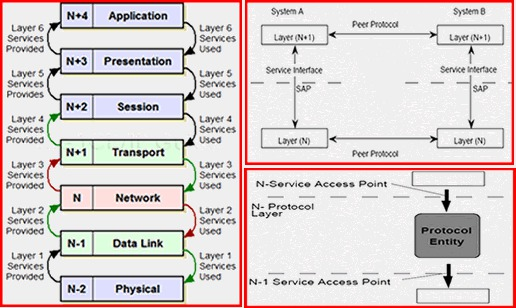
\includegraphics[width=15cm]{partie1/interaction.jpg}
\end{figure}
\begin{figure}[H]
	\centering
	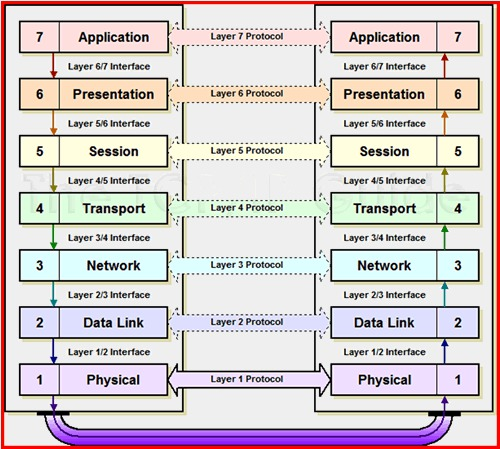
\includegraphics[width=12cm]{partie1/interaction1.jpg}
\end{figure}
\begin{figure}[H]
	\centering
	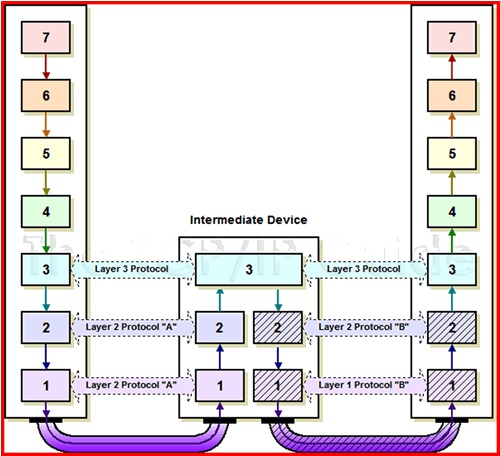
\includegraphics[width=12cm]{partie1/interaction2.jpg}
\end{figure}
\subsection{Transfert des données utilisateurs}
Les données des utilisateurs traversent toutes les couches du modèle OSI jusqu'au niveau physique qui génère le signal transmis sur le média. Chaque couche rajoute des informations de contrôle du protocole (PCI : Protocole Control Information) aux données qui lui sont passées par l'entité supérieure qui demande le service (SDU : Service Data Unit). C'est l'encapsulation des données. Cet ajout détériore les performances de débit mais sont nécessaires pour assurer les services des diféfrentes couches: adressage, contrôle d'erreurs, contrôle de flux\ldots

Cette structure est aussi appelée aussi ``structure en pelure d'oignon''.

Les données sont échangées entre les entités de même niveau qui savent les interpréter. C'est le protocole de communication qui définit le format des unités de données échangées (PDU: Protocol Data Unit) et les règles de communication.

\begin{figure}[H]
	\centering
	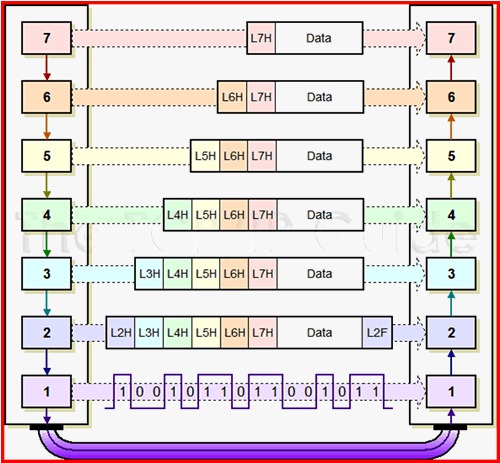
\includegraphics[width=15cm]{partie1/encapsulation.jpg}
\end{figure}

\paragraph{Segmentation/Réassemblage} Lorsque le service fourni par la couche $(N)$ fixe une limite de taille sur les données trop petites par rapport au service de la couche $(N+1)$, la couche $(N+1)$ découpe les $(N+1)-SDU$ en plusieurs fragments correspondant chacun à un $(N+1)-PDU$ avant envoi. À la réception, la couche $(N+1)$ concatène les fragments pour retrouver le $(N+1)-SDU$ initial.

\subsection{Intéractions entre entités}
Une couche donnée fournit un ensemble de services au niveau supérieur, les services sont invoqués par des primitives. Dans le Modèle OSI, les primitives sont désignées par un nom précédé de la première lettre du nom anglais de la couche. Par exemple, \texttt{$T\_$CONNECT} est une primitive de la couche Transport, \texttt{N$\_$DATA} une primitive de la couche Réseau.

Il y a 4 types de primitives de service :
\begin{itemize}
	\item Requête: une entité sollicite un service pour faire   une activité;
	\item Indication: Informe d’un évènement;
	\item Réponse: réponse à l’évènement;
	\item Confirmation: informe de la demande de service;
\end{itemize}


	\closeout\glossaireVar
	\appendix

	\chapter{Listes des annonceurs potentiels}\label{listeAnnonceurs}
Cette liste présente 48 annonceurs potentiels. Ce nombre à été retenu car, 12 créneaux de publicité étant disponibles par mois 
--- et notre solution n'étant pas connue dans les premiers temps, nous pensons que seulement un annonceur sur huit investira dans une publicité, 
ce qui nous permettrait de vendre la moitié de nos créneaux publicitaires.  

% TODO lipsum
%TODO compteur
\begin{itemize}
	\item lipsum
	\item lipsum
	\item lipsum
	\item lipsum
	\item lipsum
	\item lipsum
	\item lipsum
	\item lipsum
	\item lipsum
	\item lipsum
	\item lipsum
	\item lipsum
	\item lipsum
	\item lipsum
	\item lipsum
	\item lipsum
	\item lipsum
	\item lipsum
	\item lipsum
	\item lipsum
	\item lipsum
	\item lipsum
	\item lipsum
	\item lipsum
	\item lipsum
	\item lipsum
	\item lipsum
	\item lipsum
	\item lipsum
	\item lipsum
	\item lipsum
	\item lipsum
	\item lipsum
	\item lipsum
	\item lipsum
	\item lipsum
	\item lipsum
	\item lipsum
	\item lipsum
	\item lipsum
	\item lipsum
	\item lipsum
	\item lipsum
	\item lipsum
	\item lipsum
	\item lipsum
	\item lipsum
	\item lipsum
\end{itemize}

	\chapter[Financements et résultat]{Plans de financements et comptes de r\'esultat}
\label{tableaux}
		%plan de tr\'esorerie
		\begin{table}[h]
			\centering
			\begin{tabular}{|l|c|c|c|}
				\hline
				& {\bf N} & {\bf N+1} & {\bf N+2} \\
				\hline
			{\bf Tr\'esorerie initiale} & 0 & 19~926 & 241~350 \\
				\cline{2-4}
				{\bf Ressources} & & & \\
				- Apport des associ\'es & 75 & --- & --- \\
				- Emprunts & --- & --- & --- \\
				- CAF & 20~592 & 223~404 & 390~732 \\
				- Cessions d'immobilisations & --- & --- & --- \\
				\cline{2-4}
				{\bf Total Ressources} & 20~667 & 223~404 & 390~732 \\
				\cline{2-4}
				{\bf Emplois} & & & \\
				- Acquisitions & --- & --- & --- \\
				- Augmentation du BFR & 666 & 1~980 & 3~539 \\
				- Remboursement emprunts & --- & --- & --- \\
				- Dividendes & --- & --- & --- \\
				\cline{2-4}
				{\bf Total Emplois} & 666 & 1~980 & 3~539 \\
				\cline{2-4}
				{\bf Tr\'esorerie finale} & 19~926 & 241~350 & 628~546 \\
				\hline
			\end{tabular}
			\caption{Plan de tr\'esorerie (hypoth\`eses hautes)}
			\label{tab:planTresoH}
		\end{table}

		\begin{table}[h]
			\centering
			\begin{tabular}{|l|c|c|c|}
				\hline
				& {\bf N} & {\bf N+1} & {\bf N+2} \\
				\hline
				{\bf Tr\'esorerie initiale} & 0 & 5~971 & 52~270 \\
				\cline{2-4}
				{\bf Ressources} & & & \\
				- Apport des associ\'es & 75 & --- & --- \\
				- Emprunts & --- & --- & --- \\
				- CAF & 6~228 & 49~965 & 108~432 \\
				- Cessions d'immobilisations & --- & --- & --- \\
				\cline{2-4}
				{\bf Total Ressources} & 6~303 & 49~965 & 108~432 \\
				\cline{2-4}
				{\bf Emplois} & & & \\
				- Acquisitions & --- & --- & --- \\
				- Augmentation du BFR & 332 & 666 & 1~446 \\
				- Remboursement emprunts & --- & --- & --- \\
				- Dividendes & --- & --- & --- \\
				\cline{2-4}
				{\bf Total Emplois} & 332 & 666 & 1~446 \\
				\cline{2-4}
				{\bf Tr\'esorerie finale} & 5~971 & 52~270 & 159~256\\
				\hline
			\end{tabular}
			\caption{Plan de tr\'esorerie (hypoth\`eses basses)}
			\label{tab:planTresoB}
		\end{table}
		%compte de r\'esultat
		\vfill
		\begin{table}[h]
		  \centering
		  \begin{tabular}{|l|r|l|r|}
			\hline
			\multicolumn{4}{|c|}{\bf Compte de r\'esultat au 31/12/N}\\
			\hline
			{\bf Charges} & & {\bf Produits} & \\
			\hline
			{\bf Charges d'exploitations} & & {\bf Produits d'exploitation} & \\
			- Achat de marchandise & -- & - Vente de marchandises & --\\
			- Variation de stock & -- & - Prestation de service & 67~500\\
			- Autres charges externes & 6~408 & & \\
			- Impôts et taxes & -- & & \\
			- Charges de personnel & 40~500 & & \\
			- DAP & -- & & \\
			\cline{2-2}\cline{4-4}
			{\it Sous total 1} & 46~908 & {\it Sous total 1} & 67~500\\
			\cline{2-2}\cline{4-4}
			{\bf Charges financi\`eres} & & {\bf Produits financiers} & \\
			- Int\'er\^ets d'emprunts & -- & - Int\'er\^ets re\c cus & --\\
			- Autres & -- & - Escomptes obtenus & -- \\
			\cline{2-2}\cline{4-4}
			{\it Sous total 2} & -- & {\it Sous total 2} & -- \\
			\cline{2-2}\cline{4-4}
			{\bf Charges exceptionelles} & -- & {\bf Produits exceptionelles} & --\\
			- Dons & -- & Divers & --\\
			- Amendes et p\'enalit\'es & -- & & \\
			\cline{2-2}\cline{4-4}
			{\it Sous total 3} & -- & {\it Sous total 3} & -- \\
			\cline{2-2}\cline{4-4}
			{\bf Total des charges} & 46~908 & {\bf Total des produits} & 67~500 \\
			\cline{2-2}\cline{4-4}
			IS & 6~984 & & \\
			R\'esultat (b\'en\'efice) & 13~608 & R\'esultat (perte) & \\
			\cline{2-2}\cline{4-4}
			{\bf Total g\'en\'eral} & 67~500 & {\bf Total g\'en\'eral} & 67~500\\
			\hline
		  \end{tabular}
		  \caption{Compte de r\'esultat au terme du premier exercice (hypoth\`eses hautes)}
		  \label{tab:hypHN}
		\end{table}
		
		\begin{table}[h]
		  \centering
		  \begin{tabular}{|l|r|l|r|}
			\hline
			\multicolumn{4}{|c|}{\bf Compte de r\'esultat au 31/12/N+1}\\
			\hline
			{\bf Charges} & & {\bf Produits} & \\
			\hline
			{\bf Charges d'exploitations} & & {\bf Produits d'exploitation} & \\
			- Achat de marchandise & -- & - Vente de marchandises & --\\
			- Variation de stock & -- & - Prestation de service & 624~000\\
			- Autres charges externes & 26~196 & & \\
			- Impôts et taxes & -- & & \\
			- Charges de personnel & 374~400 & & \\
			- DAP & -- & & \\
			\cline{2-2}\cline{4-4}
			{\it Sous total 1} & 400~596 & {\it Sous total 1} & 624~000\\
			\cline{2-2}\cline{4-4}
			{\bf Charges financi\`eres} & & {\bf Produits financiers} & \\
			- Int\'er\^ets d'emprunts & -- & - Int\'er\^ets re\c cus & --\\
			- Autres & -- & - Escomptes obtenus & -- \\
			\cline{2-2}\cline{4-4}
			{\it Sous total 2} & -- & {\it Sous total 2} & -- \\
			\cline{2-2}\cline{4-4}
			{\bf Charges exceptionelles} & -- & {\bf Produits exceptionelles} & --\\
			- Dons & -- & Divers & --\\
			- Amendes et p\'enalit\'es & -- & & \\
			\cline{2-2}\cline{4-4}
			{\it Sous total 3} & -- & {\it Sous total 3} & -- \\
			\cline{2-2}\cline{4-4}
			{\bf Total des charges} & 400~596 & {\bf Total des produits} & 624~000 \\
			\cline{2-2}\cline{4-4}
			IS & 74~468 & & \\
			R\'esultat (b\'en\'efice) & 148~936 & R\'esultat (perte) & \\
			\cline{2-2}\cline{4-4}
			{\bf Total g\'en\'eral} & 624~000 & {\bf Total g\'en\'eral} & 624~000\\
			\hline
		  \end{tabular}
		  \caption{Compte de r\'esultat au terme du deuxi\`eme exercice (hypoth\`eses hautes)}
		  \label{tab:hypHN1}
		\end{table}
		
		\begin{table}[h]
		  \centering
		  \begin{tabular}{|l|r|l|r|}
			\hline
			\multicolumn{4}{|c|}{\bf Compte de r\'esultat au 31/12/N+2}\\
			\hline
			{\bf Charges} & & {\bf Produits} & \\
			\hline
			{\bf Charges d'exploitations} & & {\bf Produits d'exploitation} & \\
			- Achat de marchandise & -- & - Vente de marchandises & --\\
			- Variation de stock & -- & - Prestation de service & 1~044~000\\
			- Autres charges externes & 26~868 & & \\
			- Impôts et taxes & -- & & \\
			- Charges de personnel & 624~400 & & \\
			- DAP & -- & & \\
			\cline{2-2}\cline{4-4}
			{\it Sous total 1} & 653~268 & {\it Sous total 1} & 1~044~000\\
			\cline{2-2}\cline{4-4}
			{\bf Charges financi\`eres} & & {\bf Produits financiers} & \\
			- Int\'er\^ets d'emprunts & -- & - Int\'er\^ets re\c cus & --\\
			- Autres & -- & - Escomptes obtenus & -- \\
			\cline{2-2}\cline{4-4}
			{\it Sous total 2} & -- & {\it Sous total 2} & -- \\
			\cline{2-2}\cline{4-4}
			{\bf Charges exceptionelles} & -- & {\bf Produits exceptionelles} & --\\
			- Dons & -- & Divers & --\\
			- Amendes et p\'enalit\'es & -- & & \\
			\cline{2-2}\cline{4-4}
			{\it Sous total 3} & -- & {\it Sous total 3} & -- \\
			\cline{2-2}\cline{4-4}
			{\bf Total des charges} & 653~268 & {\bf Total des produits} & 1~044~000 \\
			\cline{2-2}\cline{4-4}
			IS & 130~244 & & \\
			R\'esultat (b\'en\'efice) & 260~488 & R\'esultat (perte) & \\
			\cline{2-2}\cline{4-4}
			{\bf Total g\'en\'eral} & 1~044~000 & {\bf Total g\'en\'eral} & 1~044~000\\
			\hline
		  \end{tabular}
		  \caption{Compte de r\'esultat au terme du troisi\`eme exercice (hypoth\`eses hautes)}
		  \label{tab:hypHN2}
		\end{table}

		\newpage
		\vfill
		\begin{table}[h]
		  \centering
		  \begin{tabular}{|l|r|l|r|}
			\hline
			\multicolumn{4}{|c|}{\bf Compte de r\'esultat au 31/12/N}\\
			\hline
			{\bf Charges} & & {\bf Produits} & \\
			\hline
			{\bf Charges d'exploitations} & & {\bf Produits d'exploitation} & \\
			- Achat de marchandise & -- & - Vente de marchandises & --\\
			- Variation de stock & -- & - Prestation de service & 45~000\\
			- Autres charges externes & 6~372 & & \\
			- Impôts et taxes & -- & & \\
			- Charges de personnel & 32~400 & & \\
			- DAP & -- & & \\
			\cline{2-2}\cline{4-4}
			{\it Sous total 1} & 38~772 & {\it Sous total 1} & 45~000\\
			\cline{2-2}\cline{4-4}
			{\bf Charges financi\`eres} & & {\bf Produits financiers} & \\
			- Int\'er\^ets d'emprunts & -- & - Int\'er\^ets re\c cus & --\\
			- Autres & -- & - Escomptes obtenus & -- \\
			\cline{2-2}\cline{4-4}
			{\it Sous total 2} & -- & {\it Sous total 2} & -- \\
			\cline{2-2}\cline{4-4}
			{\bf Charges exceptionelles} & -- & {\bf Produits exceptionelles} & --\\
			- Dons & -- & Divers & --\\
			- Amendes et p\'enalit\'es & -- & & \\
			\cline{2-2}\cline{4-4}
			{\it Sous total 3} & -- & {\it Sous total 3} & -- \\
			\cline{2-2}\cline{4-4}
			{\bf Total des charges} & 38~772 & {\bf Total des produits} & 45~000 \\
			\cline{2-2}\cline{4-4}
			IS & 2~076 & & \\
			R\'esultat (b\'en\'efice) & 4~152 & R\'esultat (perte) & \\
			\cline{2-2}\cline{4-4}
			{\bf Total g\'en\'eral} & 45~000 & {\bf Total g\'en\'eral} & 45~000\\
			\hline
		  \end{tabular}
		  \caption{Compte de r\'esultat au terme du premier exercice (hypoth\`eses basses)}
		  \label{tab:hypBN}
		\end{table}

		\vfill
		\begin{table}[h]
		  \centering
		  \begin{tabular}{|l|r|l|r|}
			\hline
			\multicolumn{4}{|c|}{\bf Compte de r\'esultat au 31/12/N+1}\\
			\hline
			{\bf Charges} & & {\bf Produits} & \\
			\hline
			{\bf Charges d'exploitations} & & {\bf Produits d'exploitation} & \\
			- Achat de marchandise & -- & - Vente de marchandises & --\\
			- Variation de stock & -- & - Prestation de service & 270~000\\
			- Autres charges externes & 25~632 & & \\
			- Impôts et taxes & -- & & \\
			- Charges de personnel & 194~400 & & \\
			- DAP & -- & & \\
			\cline{2-2}\cline{4-4}
			{\it Sous total 1} & 220~032 & {\it Sous total 1} & 270~000\\
			\cline{2-2}\cline{4-4}
			{\bf Charges financi\`eres} & & {\bf Produits financiers} & \\
			- Int\'er\^ets d'emprunts & -- & - Int\'er\^ets re\c cus & --\\
			- Autres & -- & - Escomptes obtenus & -- \\
			\cline{2-2}\cline{4-4}
			{\it Sous total 2} & -- & {\it Sous total 2} & -- \\
			\cline{2-2}\cline{4-4}
			{\bf Charges exceptionelles} & -- & {\bf Produits exceptionelles} & --\\
			- Dons & -- & Divers & --\\
			- Amendes et p\'enalit\'es & -- & & \\
			\cline{2-2}\cline{4-4}
			{\it Sous total 3} & -- & {\it Sous total 3} & -- \\
			\cline{2-2}\cline{4-4}
			{\bf Total des charges} & 220~032 & {\bf Total des produits} & 270~000 \\
			\cline{2-2}\cline{4-4}
			IS & 16~656 & & \\
			R\'esultat (b\'en\'efice) & 33~309 & R\'esultat (perte) & \\
			\cline{2-2}\cline{4-4}
			{\bf Total g\'en\'eral} & 270~000 & {\bf Total g\'en\'eral} & 270~000\\
			\hline
		  \end{tabular}
		  \caption{Compte de r\'esultat au terme du deuxi\`eme exercice (hypoth\`eses basses)}
		  \label{tab:hypBN1}
		\end{table}

		\vfill
		\begin{table}[h]
		  \centering
		  \begin{tabular}{|l|r|l|r|}
			\hline
			\multicolumn{4}{|c|}{\bf Compte de r\'esultat au 31/12/N+2}\\
			\hline
			{\bf Charges} & & {\bf Produits} & \\
			\hline
			{\bf Charges d'exploitations} & & {\bf Produits d'exploitation} & \\
			- Achat de marchandise & -- & - Vente de marchandises & --\\
			- Variation de stock & -- & - Prestation de service & 480~000\\
			- Autres charges externes & 25~968 & & \\
			- Impôts et taxes & -- & & \\
			- Charges de personnel & 345~600 & & \\
			- DAP & -- & & \\
			\cline{2-2}\cline{4-4}
			{\it Sous total 1} & 371~568 & {\it Sous total 1} & 480~000\\
			\cline{2-2}\cline{4-4}
			{\bf Charges financi\`eres} & & {\bf Produits financiers} & \\
			- Int\'er\^ets d'emprunts & -- & - Int\'er\^ets re\c cus & --\\
			- Autres & -- & - Escomptes obtenus & -- \\
			\cline{2-2}\cline{4-4}
			{\it Sous total 2} & -- & {\it Sous total 2} & -- \\
			\cline{2-2}\cline{4-4}
			{\bf Charges exceptionelles} & -- & {\bf Produits exceptionelles} & --\\
			- Dons & -- & Divers & --\\
			- Amendes et p\'enalit\'es & -- & & \\
			\cline{2-2}\cline{4-4}
			{\it Sous total 3} & -- & {\it Sous total 3} & -- \\
			\cline{2-2}\cline{4-4}
			{\bf Total des charges} & 371~568 & {\bf Total des produits} & 480~000 \\
			\cline{2-2}\cline{4-4}
			IS & 36~144 & & \\
			R\'esultat (b\'en\'efice) & 72~288 & R\'esultat (perte) & \\
			\cline{2-2}\cline{4-4}
			{\bf Total g\'en\'eral} & 480~000 & {\bf Total g\'en\'eral} & 480~000\\
			\hline
		  \end{tabular}
		  \caption{Compte de r\'esultat au terme du troisi\`eme exercice (hypoth\`eses basses)}
		  \label{tab:hypBN2}
		\end{table}


	%%% Pour insérer un mot dans le glossaire, utilisez la commande \glo{mot à apparaitre dans le texte}{Mot à apparaitre dans le glossaire}{Définition du mot} 
	\chapter{Glossaire}
	\begin{sortedlist}
		

	\end{sortedlist}
\end{document}






